\chapter{Matériels et Méthodes}

Méthode CRISP\cite{crisp}

Évaluation de nos modèles \cite{plasticc_team_2019_2539456}

\section{Compréhension du problème}

Dans cette section nous .....
Nous passerons en revue les objectifs de ce projets en termes .... et ....
Enfin nous proposerons un plan de projet.


\section{Compréhension des données}
\section{Préparation des données}\label{sec:data_preparation}
\section{Modélisation}

Les étapes précédentes nous ont permis de construire, à partir des données initiales, un dataset qui n'a plus de données manquantes et qui peut être utilisé pour entraîner des modèles de prédictions. Nous avons basé notre modélisation sur deux principales classes de modèles:
\begin{itemize}
    \item \textbf{Les modèles basés sur les caractéristiques :} Il s'agit ici de modèles qui se basent sur les méta données et sur les caractéristiques telles que la moyenne, les quartiles, la valeur maximale, la valeur minimale et bien d'autres pour faire les prédictions. Ces modèles supposent que les séries d'une même classes ont des caractéristiques similaires tandis que les séries de classes différentes ont des caractéristiques qui ne sont pas similaires.
    \item \textbf{Les modèles basés sur les similarités à des sous séries:} Ces modèles se basent sur l'hypothèse qu'il y a dans les séries temporelles des sous séquences qui sont représentatives pour la classes; ces sous-séquences sont appelées \textbf{shapelets} \citep{ye2009time}.
\end{itemize}
La figure \ref{fig:modeling_shema} est une représentation schématique du processus de modélisation que nous avons implémenté. Ce schéma va de l'acquisition des données jusqu'au modèle de prédiction. L'étape \textit{preprocessing} correspond à l'étape de préparation des données (Section \ref{sec:data_preparation}) dont le but était le traitement des valeurs manquantes et la normalisation des données. Les éléments suivant seront expliqués dans les lignes qui suivent selon qu'on soit orienté caractéristiques (Section \ref{sec:feature_based_model}) ou shapelet (Section \ref{sec:shapelet_based_model})

\begin{figure}[h]
    \centering
    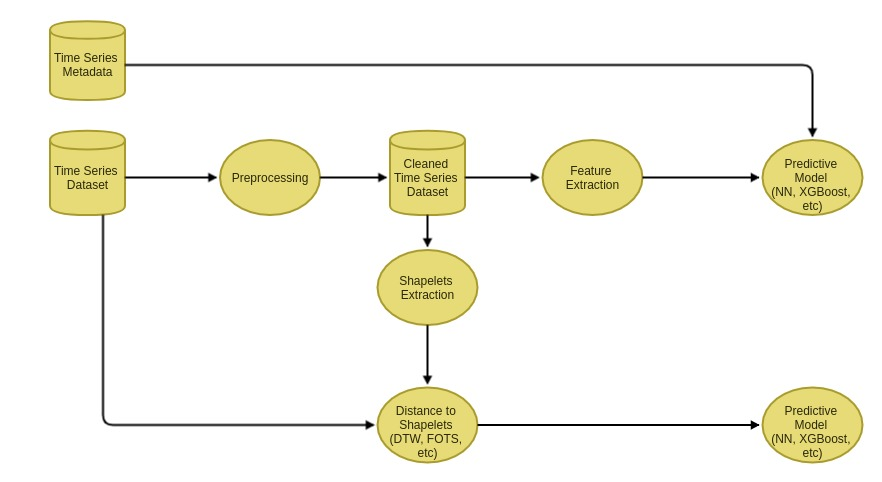
\includegraphics[width=15cm]{report/figures/modeling-schema.jpg}
    \caption{Schéma générale de modélisation}
    \label{fig:modeling_shema}
\end{figure}

\subsection{Modèles basés sur les caractéristiques}\label{sec:feature_based_model}

\subsection{Modèles basés sur les shapelets}\label{sec:shapelet_based_model}
Un Shapelet est défini comme une sous-séquence d'une série temporelle qui est représentative pour la classe \citep{ye2009time}. Ainsi une série temporelle appartient à une classe donnée si elle contient le \textit{shapelet} représentatif de ladite classe. Dans la pratique les séries d'une même classe n'ont pas exactement les mêmes sous-séquences représentatives mais elles ont des sous-séquences qui sont similaires aux sous-séquences représentatives de la classe. 
La classification des séries temporelles peut être réalisée par un arbre de décision dans lequel l'attribut de division (split) à chaque noeud est un \textit{shapelet} et les données sont séparées en fonction de la similarité à ce \textit{shapelet}.

\section{Évaluation}
\section{Déploiement}